% Created 2013-05-16 Thu 10:41
\documentclass[11pt,a4paper]{article}
\usepackage[T1]{fontenc}
\usepackage{fontspec}
\usepackage{graphicx}
\defaultfontfeatures{Mapping=tex-text}
\setmainfont{DejaVu Sans}
\setmonofont[Scale=0.8]{FreeMono}
\usepackage{geometry}
\geometry{a4paper, textwidth=6.5in, textheight=10in,
            marginparsep=7pt, marginparwidth=.6in}
\usepackage[usenames,dvipsnames]{xcolor}
\usepackage[bookmarks, colorlinks, breaklinks]{hyperref}
\hypersetup{linkcolor=black, citecolor=blue,filecolor=black,urlcolor=MidnightBlue}
\pagestyle{empty}
\usepackage{amsmath}

\providecommand{\alert}[1]{\textbf{#1}}

\title{Animal classification decision tree}
\author{Chris Perivolaropulos}
\date{\today}
\hypersetup{
  pdfkeywords={},
  pdfsubject={},
  pdfcreator={Emacs Org-mode version 7.9.2}}

\begin{document}

\maketitle

\setcounter{tocdepth}{3}
\tableofcontents
\vspace*{1cm}

\section{Animal classification decision tree}
\label{sec-1}
\subsection{Part A}
\label{sec-1-1}

   To generate the type selection decision tree I used the J48 algorithm.

   \begin{figure}[htb]
   \centering
   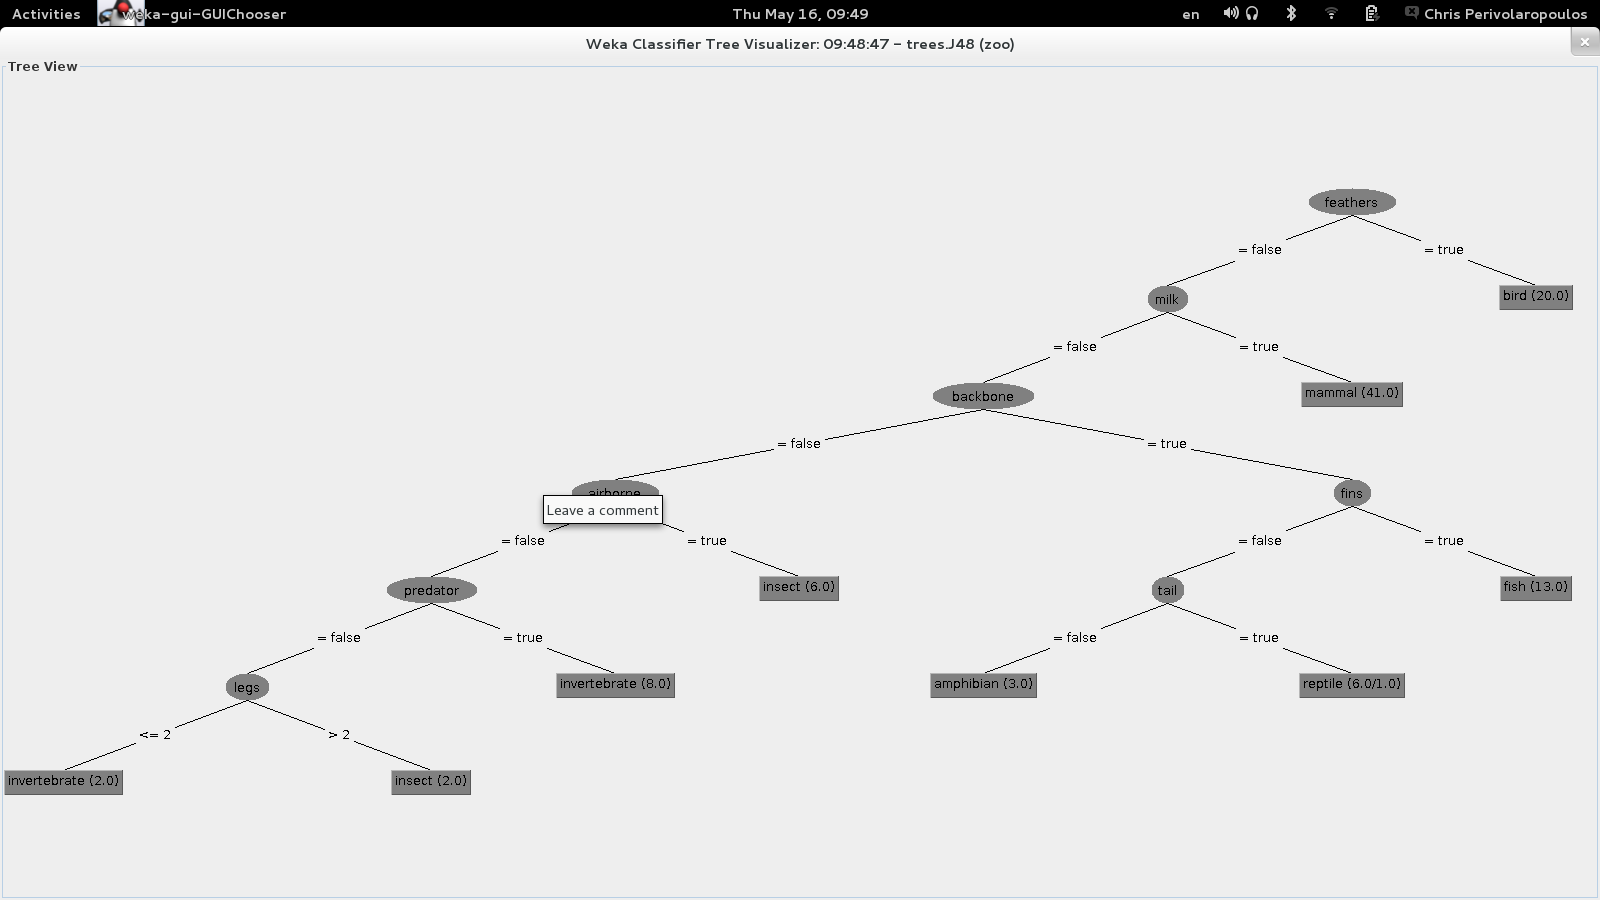
\includegraphics[width=.9\linewidth]{./animaltree.png}
   \caption{Animal decision tree.}
   \end{figure}


   A textual form of the tree is easier to manipulate.


\begin{verbatim}
feathers = false
|   milk = false
|   |   backbone = false
|   |   |   airborne = false
|   |   |   |   predator = false
|   |   |   |   |   legs <= 2: invertebrate (2.0)
|   |   |   |   |   legs > 2: insect (2.0)
|   |   |   |   predator = true: invertebrate (8.0)
|   |   |   airborne = true: insect (6.0)
|   |   backbone = true
|   |   |   fins = false
|   |   |   |   tail = false: amphibian (3.0)
|   |   |   |   tail = true: reptile (6.0/1.0)
|   |   |   fins = true: fish (13.0)
|   milk = true: mammal (41.0)
feathers = true: bird (20.0)
\end{verbatim}

   Then save all of the attributes in a file called attributes.


\begin{verbatim}
animal
hair
feathers
eggs
milk
airborne
aquatic
predator
toothed
backbone
breathes
venomous
fins
legs
tail
domestic
catsize
type
\end{verbatim}

   Then run we run


\begin{verbatim}
$ cat tree | sed 's/[\t |]*\([^ \t]*\) [=<>].*/\1/' | sort | uniq | cat attributes - | sort | uniq -u
\end{verbatim}

   What this does basically is it extracts the attributes from the
   textual tree using \texttt{sed}, then it cuts out the duplicate lines
   with \texttt{sort | uniq} then appends the attributes to stdout from the
   \texttt{attributes} file and sorts the lines. Now we know the attributes
   we have used are the ones that are double so we \texttt{uniq -u} to leave
   them out. The result is:


\begin{verbatim}
animal
aquatic
breathes
catsize
domestic
eggs
hair
toothed
type
venomous
\end{verbatim}

   Ignore those (except \texttt{type}) in weka and as expected the tree is
   unchanged.
\subsection{Part B}
\label{sec-1-2}

   We use the BayesNet algorithm. Attempting to extract the figure we
   notice weka exports erronous dot code. Nothing too serious, just
   remove dots and dashes from graph and node names. Long story short
   this is what we come up with.

   \begin{figure}[htb]
   \centering
   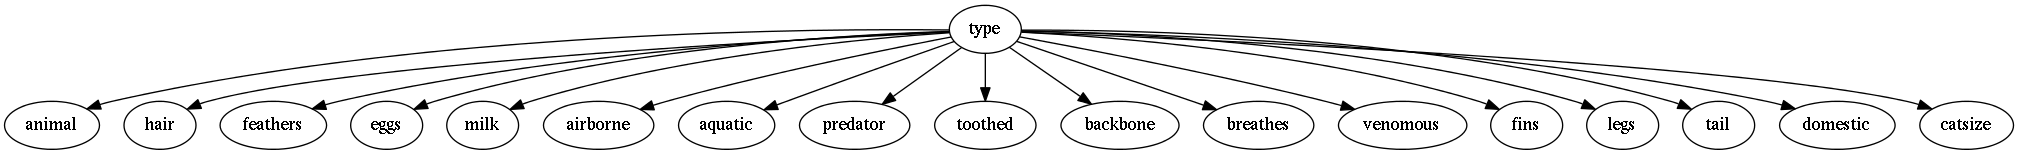
\includegraphics[width=.9\linewidth]{./bayes.png}
   \caption{Bayes networg as generated by weka.}
   \end{figure}

   Apparently weka has included all attributes to the bayesian
   network. Also it isn't trivial to get the Probability Distribution
   Tables in the graph. To make a decision, we minimize the
   probability of that decision being untrue based on the PDTs
   therefore removing any attribute would obviously remove it from the
   bayes network.
\subsection{Part C}
\label{sec-1-3}

   I wasn't able to set the number of clusters to use. The results
   weka came up with were:

\begin{verbatim}
=== Run information ===

Scheme:       weka.clusterers.SimpleKMeans -N 2 -A "weka.core.EuclideanDistance -R first-last" -I 500 -num-slots 1 -S 10
Relation:     zoo-weka.filters.unsupervised.attribute.Remove-R18
Instances:    101
Attributes:   17
           animal
           hair
           feathers
           eggs
           milk
           airborne
           aquatic
           predator
           toothed
           backbone
           breathes
           venomous
           fins
           legs
           tail
           domestic
           catsize
Test mode:    evaluate on training data


=== Clustering model (full training set) ===


kMeans
======

Number of iterations: 2
Within cluster sum of squared errors: 384.16399263211383
Missing values globally replaced with mean/mode

Cluster centroids:
                      Cluster#
Attribute    Full Data          0          1
              (101)       (41)       (60)
============================================
animal            frog   aardvark       frog
hair             false       true      false
feathers         false      false      false
eggs              true      false       true
milk             false       true      false
airborne         false      false      false
aquatic          false      false      false
predator          true       true       true
toothed           true       true      false
backbone          true       true       true
breathes          true       true       true
venomous         false      false      false
fins             false      false      false
legs            2.8416     3.3659     2.4833
tail              true       true       true
domestic         false      false      false
catsize          false       true      false




Time taken to build model (full training data) : 0 seconds

=== Model and evaluation on training set ===

Clustered Instances

0       41 ( 41%)
1       60 ( 59%)
\end{verbatim}


\begin{verbatim}
=== Run information ===

Scheme:       weka.clusterers.EM -I 100 -N -1 -X 10 -max -1 -ll-cv 1.0E-6 -ll-iter 1.0E-6 -M 1.0E-6 -num-slots 1 -S 100
Relation:     zoo-weka.filters.unsupervised.attribute.Remove-R18
Instances:    101
Attributes:   17
           animal
           hair
           feathers
           eggs
           milk
           airborne
           aquatic
           predator
           toothed
           backbone
           breathes
           venomous
           fins
           legs
           tail
           domestic
           catsize
Test mode:    evaluate on training data


=== Clustering model (full training set) ===


EM
==

Number of clusters selected by cross validation: 6
Number of iterations performed: 3


           Cluster
Attribute           0        1        2        3        4        5
                   (0.18)    (0.2)   (0.08)   (0.16)   (0.19)    (0.2)
===================================================================
animal
aardvark           1   1.0423        1        1   1.9576        1
antelope           1   1.9741        1        1   1.0259        1
bass               1        1   1.0003   1.9997        1        1
bear               1   1.0423        1        1   1.9576        1
boar               1   1.0795        1        1   1.9205        1
buffalo            1   1.9741        1        1   1.0259        1
calf               1   1.9921        1        1   1.0079        1
carp               1        1   1.0002   1.9998        1        1
catfish            1        1   1.0003   1.9997        1        1
cavy               1   1.9968        1        1   1.0031        1
cheetah            1   1.0795        1        1   1.9205        1
chicken            1        1        1        1        1        2
chub               1        1   1.0003   1.9997        1        1
clam          1.9988        1   1.0011        1        1        1
crab          1.9977        1   1.0022        1        1        1
crayfish      1.9994        1   1.0006        1        1        1
crow               1        1        1        1        1        2
deer               1   1.9741        1        1   1.0259        1
dogfish            1        1   1.0001   1.9999        1        1
dolphin            1        1   1.0026    1.872   1.1255        1
dove               1        1        1        1        1        2
duck               1        1        1        1        1        2
elephant           1   1.9741        1        1   1.0259        1
flamingo           1        1        1        1        1        2
flea          1.9993        1   1.0007        1        1        1
frog          1.0022        1   2.9969   1.0009   1.0001        1
fruitbat           1   1.9769   1.0001        1    1.004   1.0191
giraffe            1   1.9741        1        1   1.0259        1
girl               1   1.0588        1        1   1.9411        1
gnat          1.9998        1   1.0002        1        1        1
goat               1   1.9921        1        1   1.0079        1
gorilla            1   1.8837   1.0001        1   1.1162   1.0001
gull               1        1        1        1        1        2
haddock            1        1   1.0003   1.9997        1        1
hamster            1   1.9983        1        1   1.0017        1
hare               1   1.9945        1        1   1.0055        1
hawk               1        1        1        1        1        2
herring            1        1   1.0003   1.9997        1        1
honeybee      1.9999        1   1.0001        1        1        1
housefly      1.9999        1   1.0001        1        1        1
kiwi               1        1        1        1        1        2
ladybird      1.9996        1   1.0004        1        1        1
lark               1        1        1        1        1        2
leopard            1   1.0795        1        1   1.9205        1
lion               1   1.0795        1        1   1.9205        1
lobster       1.9994        1   1.0006        1        1        1
lynx               1   1.0795        1        1   1.9205        1
mink               1   1.0104        1        1   1.9895        1
mole               1   1.3479   1.0002        1   1.6519        1
mongoose           1   1.0795        1        1   1.9205        1
moth          1.9999        1   1.0001        1        1        1
newt          1.0002        1   1.9892   1.0105   1.0002        1
octopus       1.9998        1   1.0002        1        1        1
opossum            1   1.3479   1.0002        1   1.6519        1
oryx               1   1.9741        1        1   1.0259        1
ostrich            1        1        1        1        1        2
parakeet           1        1        1        1        1        2
penguin            1        1        1        1        1        2
pheasant           1        1        1        1        1        2
pike               1        1   1.0001   1.9999        1        1
piranha            1        1   1.0003   1.9997        1        1
pitviper      1.0002        1   1.9844   1.0154        1        1
platypus      1.0001   1.0023    1.006        1   1.9916        1
polecat            1   1.0795        1        1   1.9205        1
pony               1   1.9921        1        1   1.0079        1
porpoise           1        1   1.0026    1.872   1.1255        1
puma               1   1.0795        1        1   1.9205        1
pussycat           1   1.2575        1        1   1.7425        1
raccoon            1   1.0795        1        1   1.9205        1
reindeer           1   1.9921        1        1   1.0079        1
rhea               1        1        1        1        1        2
scorpion      1.9965        1   1.0035        1        1        1
seahorse           1        1   1.0003   1.9997        1        1
seal               1        1   1.0004   1.0034   1.9962        1
sealion            1    1.001        1   1.0004   1.9985        1
seasnake           1        1   1.0153   1.9847        1        1
seawasp       1.9962        1   1.0031   1.0006        1        1
skimmer            1        1        1        1        1        2
skua               1        1        1        1        1        2
slowworm      1.0003        1   1.9654   1.0342   1.0001        1
slug          1.9974        1   1.0026        1        1        1
sole               1        1   1.0003   1.9997        1        1
sparrow            1        1        1        1        1        2
squirrel           1   1.9861   1.0001        1    1.013   1.0009
starfish      1.9987        1   1.0013        1        1        1
stingray           1        1   1.0002   1.9998        1        1
swan               1        1        1        1        1        2
termite       1.9993        1   1.0007        1        1        1
toad          1.0045        1   1.9946   1.0009        1        1
tortoise      1.0367   1.0028   1.9588   1.0005   1.0012        1
tuatara       1.0003   1.0001   1.9981   1.0009   1.0006        1
tuna               1        1   1.0001   1.9999        1        1
vampire            1   1.9769   1.0001        1    1.004   1.0191
vole               1   1.9945        1        1   1.0055        1
vulture            1        1        1        1        1        2
wallaby            1   1.9378        1        1   1.0619   1.0003
wasp          1.9999        1   1.0001        1        1        1
wolf               1   1.0795        1        1   1.9205        1
worm          1.9974        1   1.0026        1        1        1
wren               1        1        1        1        1        2
[total]     118.0237 120.4673 107.9382 115.7936 118.7378 120.0395
hair
false        15.0238   1.0029   8.9305  16.7897    1.253       21
true          4.9998  21.4644   1.0077   1.0039  19.4847   1.0395
[total]      20.0237  22.4673   9.9382  17.7936  20.7378  22.0395
feathers
false        19.0237  21.4673   8.9382  16.7936  19.7378   1.0395
true               1        1        1        1        1       21
[total]      20.0237  22.4673   9.9382  17.7936  20.7378  22.0395
eggs
false         1.9965  21.4621   1.0253   3.7325  18.7441   1.0395
true         18.0271   1.0052   8.9129  14.0611   1.9937       21
[total]      20.0237  22.4673   9.9382  17.7936  20.7378  22.0395
milk
false        19.0236   1.0029   8.9256  15.0458   1.0021       21
true          1.0001  21.4644   1.0125   2.7478  19.7356   1.0395
[total]      20.0237  22.4673   9.9382  17.7936  20.7378  22.0395
airborne
false        13.0245  19.5136   8.9373  16.7936  19.7299   5.0013
true          6.9992   2.9538   1.0009        1   1.0079  17.0382
[total]      20.0237  22.4673   9.9382  17.7936  20.7378  22.0395
aquatic
false        13.0255  21.4536   4.9198    1.051  15.5107  15.0395
true          6.9982   1.0138   5.0184  16.7425   5.2271        7
[total]      20.0237  22.4673   9.9382  17.7936  20.7378  22.0395
predator
false        10.0341  19.5615   2.9619   5.0003   1.4027  12.0394
true          9.9895   2.9058   6.9763  12.7932   19.335  10.0001
[total]      20.0237  22.4673   9.9382  17.7936  20.7378  22.0395
toothed
false        19.0159   1.0051   1.9849   1.0013   1.9928       21
true          1.0078  21.4623   7.9532  16.7923   18.745   1.0395
[total]      20.0237  22.4673   9.9382  17.7936  20.7378  22.0395
backbone
false        18.9791        1   1.0202   1.0007        1        1
true          1.0445  21.4673    8.918  16.7929  19.7378  21.0395
[total]      20.0237  22.4673   9.9382  17.7936  20.7378  22.0395
breathes
false         7.9901        1   1.0274  14.9825        1        1
true         12.0336  21.4673   8.9108   2.8111  19.7378  21.0395
[total]      20.0237  22.4673   9.9382  17.7936  20.7378  22.0395
venomous
false        15.0299  21.4673   6.9328  14.7928  19.7377  21.0395
true          4.9938        1   3.0054   3.0008        1        1
[total]      20.0237  22.4673   9.9382  17.7936  20.7378  22.0395
fins
false        19.0237  21.4663   8.9298   2.0487  17.4921  21.0395
true               1    1.001   1.0084  15.7449   3.2457        1
[total]      20.0237  22.4673   9.9382  17.7936  20.7378  22.0395
legs
mean          4.7221   3.5289   3.0036   0.0035   3.5055        2
std. dev.     2.6584   0.8487   1.7359   0.1185     1.13   2.0334

tail
false        17.9893    3.024   4.0086   1.0059   4.9721   1.0001
true          2.0344  19.4433   5.9295  16.7877  15.7657  21.0394
[total]      20.0237  22.4673   9.9382  17.7936  20.7378  22.0395
domestic
false        18.0237  15.1873   8.9378  15.7938  18.0179  18.0395
true          1.9999   7.2801   1.0004   1.9998   2.7198        4
[total]      20.0237  22.4673   9.9382  17.7936  20.7378  22.0395
catsize
false         17.987   8.6198   7.9669  11.0458   2.3413  15.0391
true          2.0366  13.8475   1.9713   6.7478  18.3964   7.0004
[total]      20.0237  22.4673   9.9382  17.7936  20.7378  22.0395


Time taken to build model (full training data) : 1.18 seconds

=== Model and evaluation on training set ===

Clustered Instances

0       18 ( 18%)
1       19 ( 19%)
2        8 (  8%)
3       16 ( 16%)
4       20 ( 20%)
5       20 ( 20%)


Log likelihood: -10.54745
\end{verbatim}

   EM did a much better job than k-means.

\end{document}
